\documentclass[10pt]{beamer}

%% Based on the original theme by Matthias Vogelgesang

\usetheme[progressbar=frametitle]{metropolis}
\usepackage{appendixnumberbeamer}

\usepackage{booktabs}
\usepackage{multicol}
\usepackage[scale=2]{ccicons}
\usepackage{amsmath}


\usepackage{graphicx,threeparttable,caption}
\captionsetup{justification=raggedright,singlelinecheck=false}
\captionsetup[table]{labelsep=space}

%\usepackage{pgfplots}
%\usepgfplotslibrary{dateplot}

% \usepackage{background}
% \backgroundsetup{
%     placement=center,
%     scale=8,
%     contents={DRAFT},
%     opacity=1.5
% }
% \setbeamertemplate{background}{\BgMaterial}

\usepackage{xspace}
\newcommand{\themename}{\textbf{\textsc{metropolis}}\xspace}


\usepackage[style=apa, sortcites=true, sorting=nyt, backend=biber]{biblatex}
\DeclareLanguageMapping{american}{american-apa}

%% adding bibliography file to list of resources
\addbibresource{bibliography.bib}

\usepackage[export]{adjustbox}
\graphicspath{ {./images/} }



%%%%%%%%%%%%%%%%%%%%%%%%%%%%
%% UNCC Theme Adjustments %%
%%%%%%%%%%%%%%%%%%%%%%%%%%%%
\definecolor{CanvasBG}{HTML}{FAFAFA}

% From the official style guide
\definecolor{UnccGreen}{HTML}{00703C}
\definecolor{UnccGold}{HTML}{B3A369}
\definecolor{UnccLightGreen}{HTML}{C3D7A4}
\definecolor{UnccYellow}{HTML}{F0CB00}
\definecolor{UnccOrange}{HTML}{F3901D}
\definecolor{UnccLightYellow}{HTML}{FFF6DC}
\definecolor{UnccBlue}{HTML}{00728F}
\definecolor{UnccPink}{HTML}{DE3A6E}
\definecolor{White}{HTML}{FFFFFF}
\definecolor{LightGray}{HTML}{DDDDDD}

% Supporting Color Palette
\definecolor{WarmGray}{HTML}{696158}
\definecolor{StoneGray}{HTML}{717C7D}
\definecolor{DarkGreen}{HTML}{2C5234}
\definecolor{LightGreen}{HTML}{509E2F}
\definecolor{BrightGold}{HTML}{F0CB00}

% Screamers
\definecolor{Royal}{HTML}{72246C}
\definecolor{Ocean}{HTML}{006BA6}
\definecolor{Flash}{HTML}{B52555}
\definecolor{Citrus}{HTML}{FFB81C}
\definecolor{Spring}{HTML}{CEDC00}

% Serenity
\definecolor{Garden}{HTML}{B7CE95}
\definecolor{Sand}{HTML}{F0E991}
\definecolor{Bloom}{HTML}{F1E6B2}
\definecolor{Clay}{HTML}{B7B09C}
\definecolor{Cloud}{HTML}{BAC5B9}

% Set colors here
\setbeamercolor{frametitle}{bg=UnccGreen}
\setbeamercolor{progress bar}{bg=BrightGold, fg=UnccGreen}
\setbeamercolor{alerted text}{fg=Flash}

\setbeamercolor{block title}{bg=LightGreen, fg=White}
\setbeamercolor{block title example}{bg=Ocean, fg=White}
\setbeamercolor{block title alerted}{bg=Citrus, fg=White}
\setbeamercolor{block body}{bg=CanvasBG}

\metroset{titleformat=smallcaps, progressbar=foot}

\makeatletter
\setlength{\metropolis@progressinheadfoot@linewidth}{2pt}
\setlength{\metropolis@titleseparator@linewidth}{2pt}
\setlength{\metropolis@progressonsectionpage@linewidth}{2pt}
%%%%%%%%%%%%%%%%%%%%%%%%%%%%
%% UNCC Theme Adjustments %%
%%%%%%%%%%%%%%%%%%%%%%%%%%%%


\title{Sprint 2}
\subtitle{College and Career Readiness in Charlotte, NC: An Analysis on Academic Performance, Career Readiness, and Upward Mobility.}
% \date{\today}
\date{February 9, 2022}
\author{Khem Khadka \and Cody Scott \and Joshua Hernandez}
\institute{DTSC 4301 \\ School of Data Science \\ University of North Carolina at Charlotte}
\titlegraphic{\vspace{4.5cm}\flushright\includegraphics[height=3cm]{UNC_Logo.png}}

\begin{document}

\maketitle

\begin{frame}{Table of contents}
  \setbeamertemplate{section in toc}[sections numbered]
  \tableofcontents[hideallsubsections]
\end{frame}

\section[Overview]{Background}

\begin{frame}[fragile]{Project Overview}
    \fontsize{11pt}{7.2}
    \begin{itemize}
        \setlength\itemsep{2em}
        \item Out of 50 largest cities in the United States, Charlotte ranks last in upward economic mobility
        \item Leading On Opportunity Task Force worked with experts and communities to recommend structural changes to improve mobility
    \end{itemize}
\end{frame}

\begin{frame}
    \begin{figure}
        \caption{}
        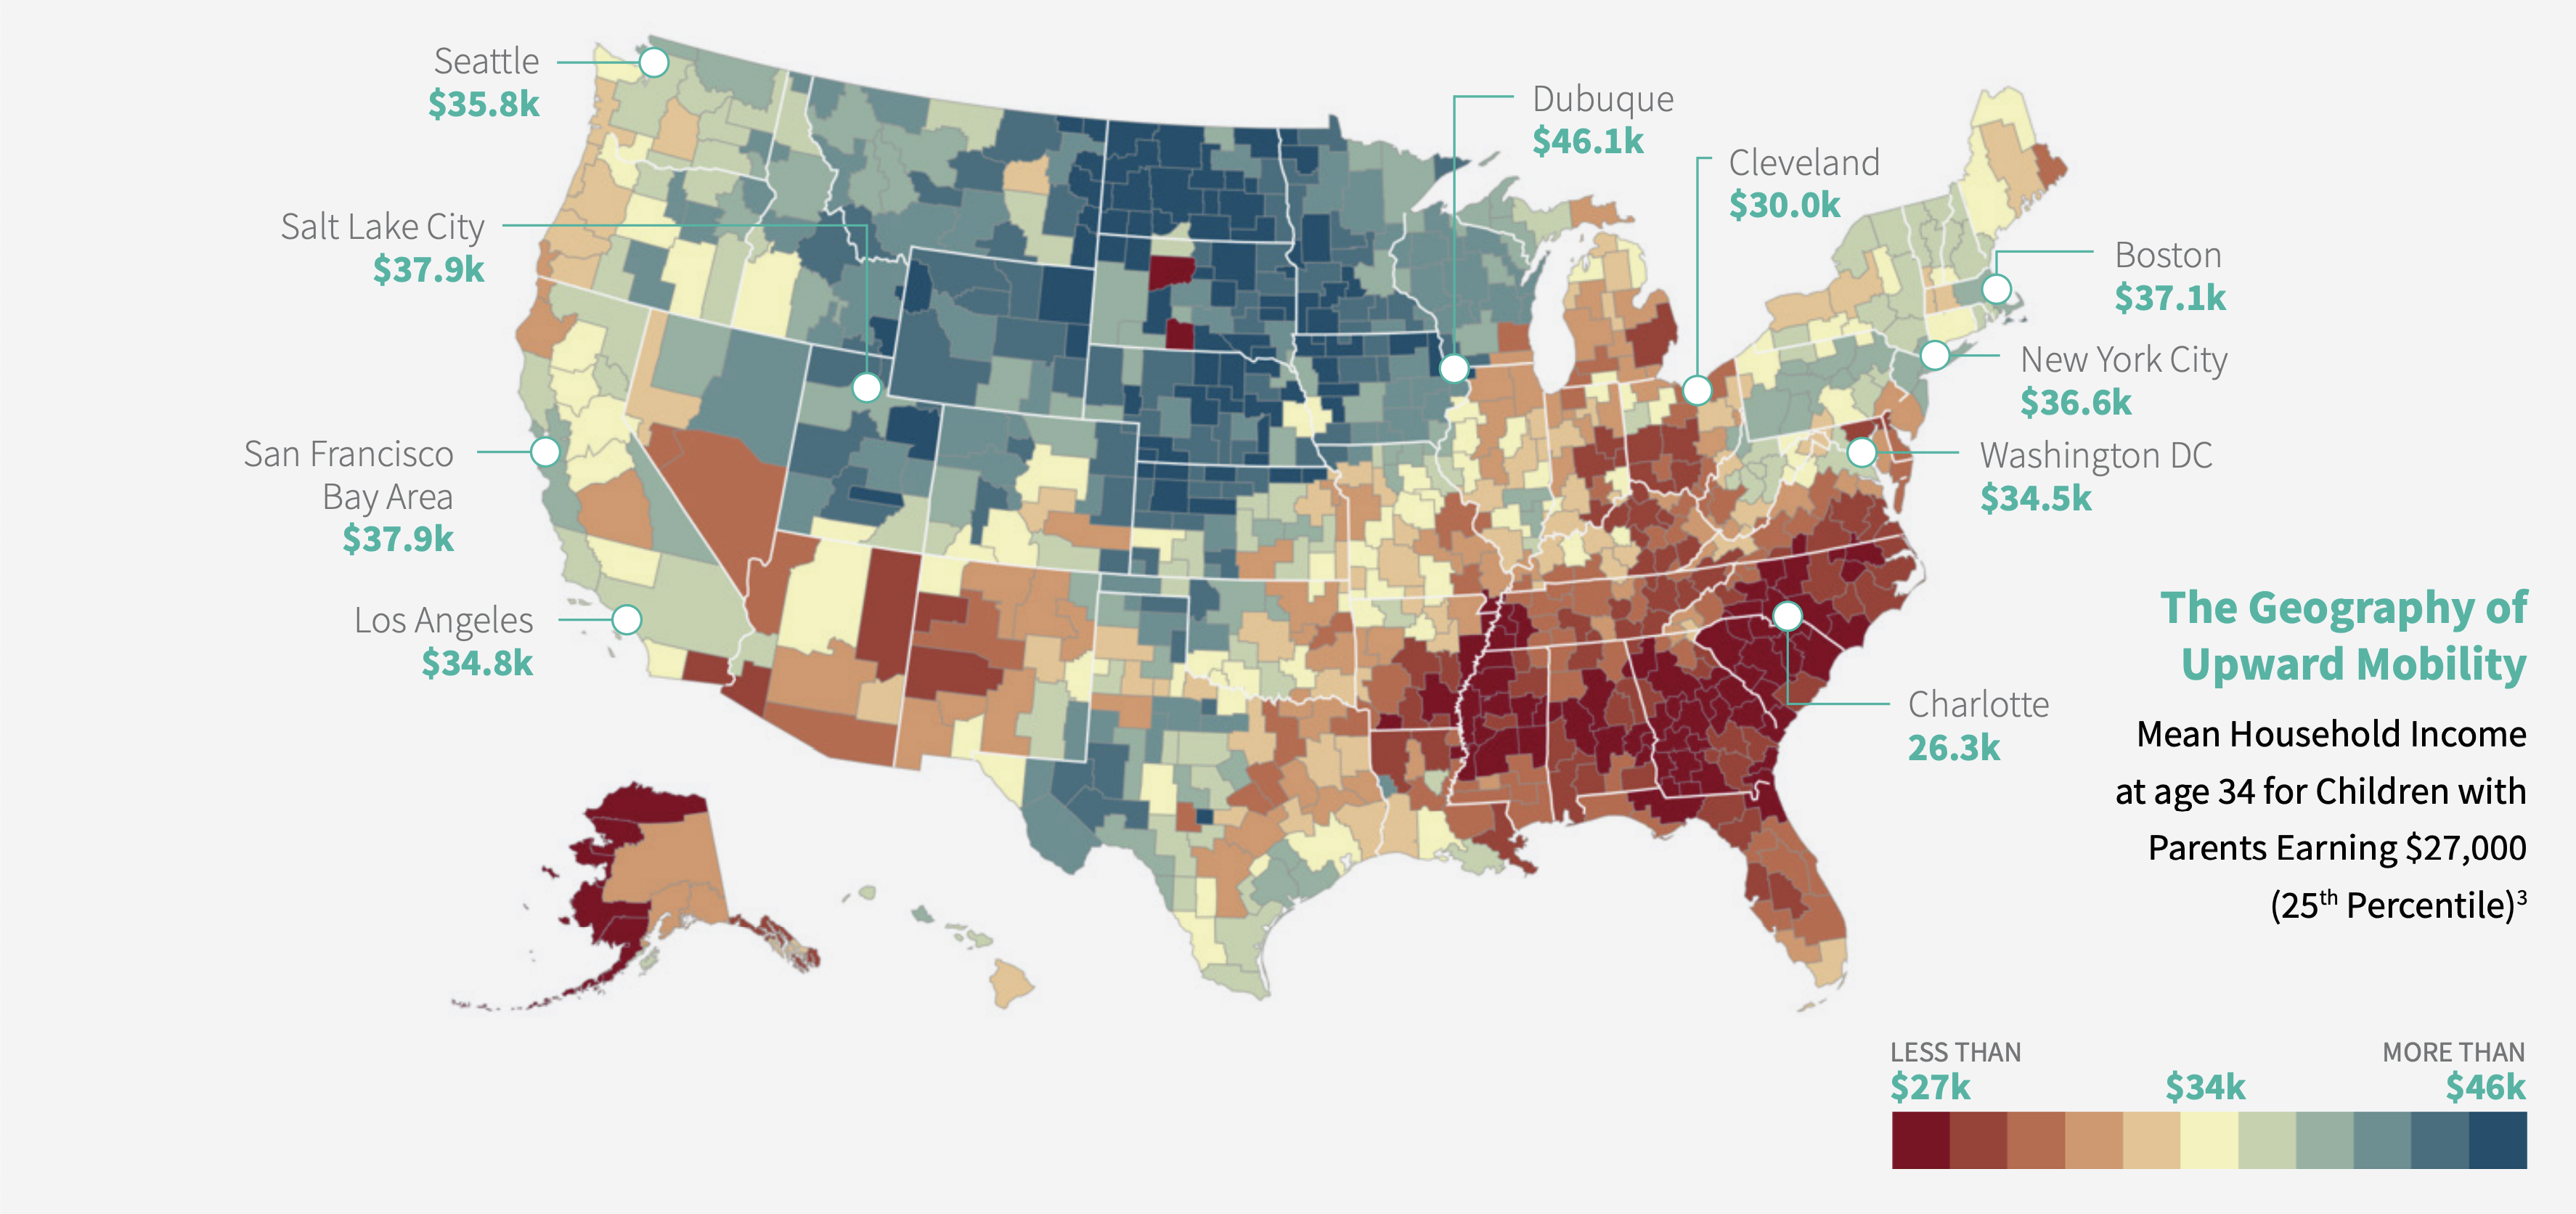
\includegraphics[width=10cm]{LOO_Chart.png}
        \label{fig6}
    \end{figure}
    Source: Chetty Report, \href{https://academic.oup.com/qje/article/129/4/1553/1853754?login=true}{2014}
\end{frame}

\begin{frame}
    \begin{figure}
        \caption{}
        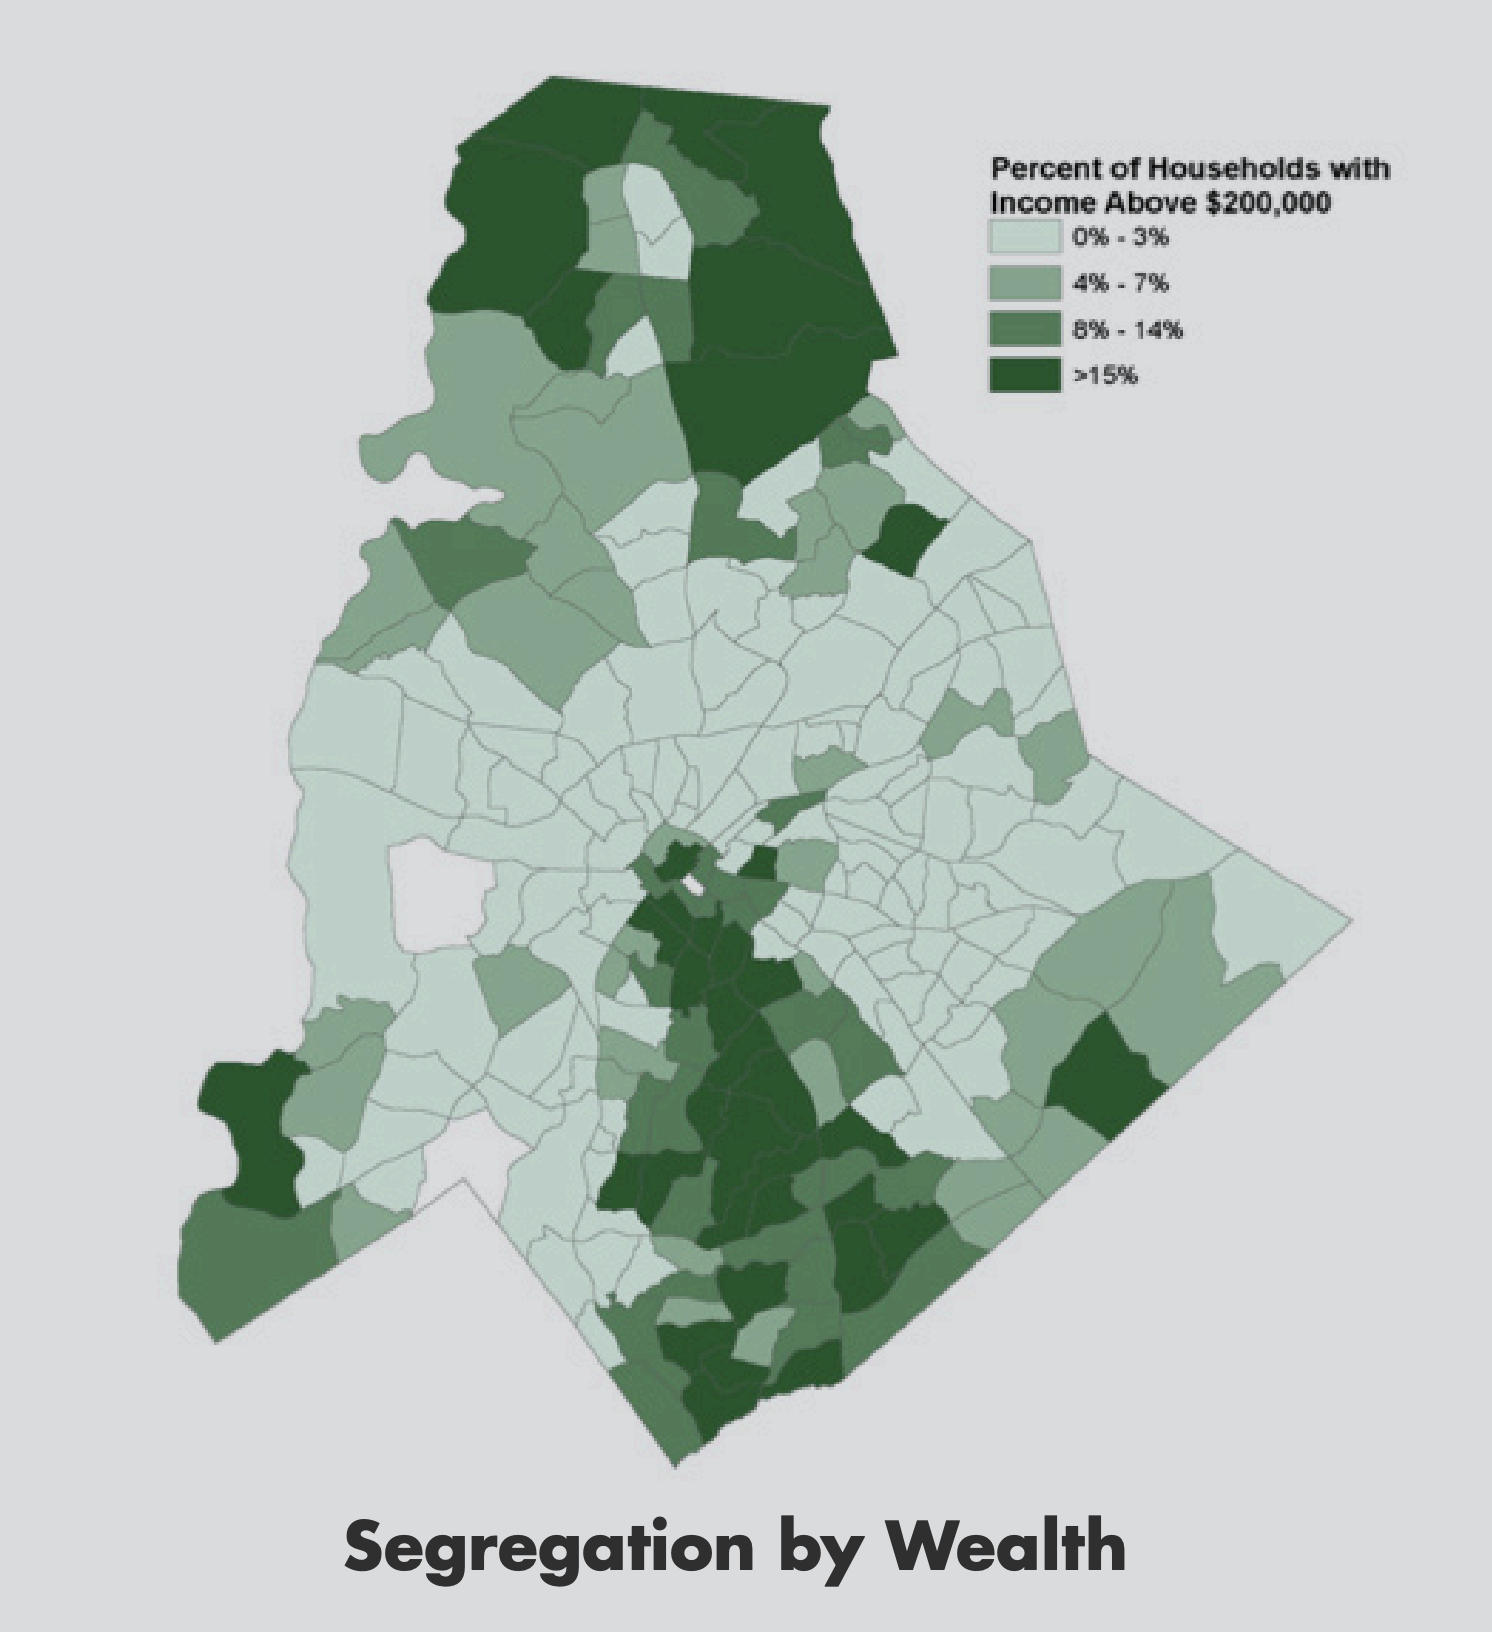
\includegraphics[height=7cm]{Chetty_Chart.png}
        \label{fig7}
    \end{figure}
    Source: Leading on Opportunity Report, \href{https://s3.amazonaws.com/static.leadingonopportunity.org/downloads/LeadingOnOpportunity_Report-Compressed.pdf}{2017}
\end{frame}

\subsection[Research Question]{Research Question}

\begin{frame}{Research Question}
    \fontsize{12pt}{7.2}
    \large{\textsc{Will the recommendations made from the task force show a positive effect on minority children, and children from low economic statuses in educational performance, college readiness, or career readiness?}}

\end{frame}

\section[Hypotheses]{Hypotheses}

\begin{frame}[fragile]{Hypotheses}
    \fontsize{11pt}{7.2}
    \begin{block}{Hypothesis 1}
        As the number and quality of mentors increase, there will be an increase in academic performance and college acceptance rates for low-socioeconomic students.
    \end{block}

    \pause

    \vspace{.6cm}

    \begin{exampleblock}{Variables}
        \begin{itemize}
            \item[$\triangleright$] AP Participation Rate
            \item[$\triangleright$] AP Passing Rate
            \item[$\triangleright$] College Enrollment Rate 
            \item[$\triangleright$] Total Guidance Counselors in Charlotte-Mecklenburg Schools
            \item[$\triangleright$] Quality of Mentor Bias Training
        \end{itemize}
    \end{exampleblock}

\end{frame}

\begin{frame}[fragile]{Hypotheses}
    \fontsize{11pt}{7.2}
    \begin{block}{Hypothesis 2}
        As the quality and number of mentors increase, there will be an increase in obtained CTE  Credentials by students within Charlotte Mecklenburg County Schools.
    \end{block}

    \pause 

    \vspace{1cm}

    \begin{exampleblock}{Variables}
        \begin{itemize}
            \item[$\triangleright$] Career and Technical Education Enrollment
            \item[$\triangleright$] Career and Technical Education Credentials
            \item[$\triangleright$] Total Guidance Counselors in Charlotte-Mecklenburg Schools
            \item[$\triangleright$] Quality of Mentor Bias Training
        \end{itemize}
    \end{exampleblock}

\end{frame}

\begin{frame}[fragile]{Hypotheses Model}

    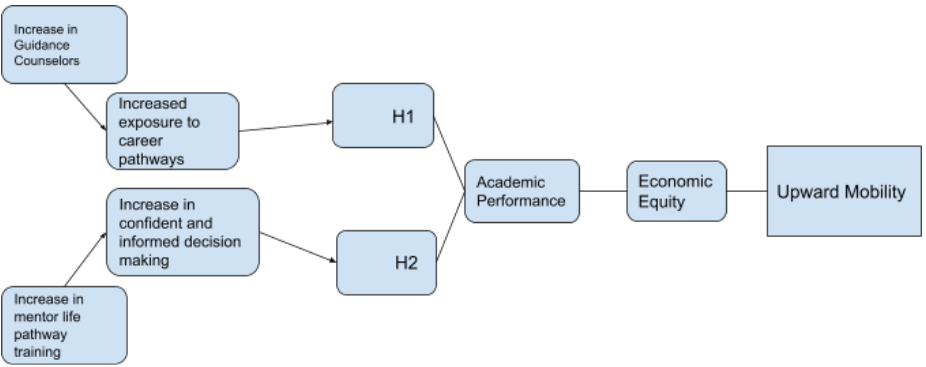
\includegraphics[width=11.4cm]{Hypothesis_Modelv2.png}

\end{frame}


\section[Data Sources]{Data Sources}

\begin{frame}{Data Sources}
    \fontsize{11pt}{7.2}
    \begin{exampleblock}{Sources}
        \begin{itemize}
            \setlength\itemsep{3mm}
            \item[$\triangleright$] North Carolina Department of Public Instruction
                \begin{itemize}
                    \item North Carolina School Report Cards
                    \item North Carolina Public Schools Statistical Profile
                    \item The Educational Directory and Demographical Information Exchange (EDDIE)
                \end{itemize}
            \item[$\triangleright$] The National Center for Education Statistics 
                \begin{itemize}
                    \item Education Demographics and Geographic Estimates on School Neighborhood Poverty
                \end{itemize}
            \item[$\triangleright$] Charlotte Open Data Portal
                \begin{itemize}
                    \item 2019 Median Household Income by school Zip Code
                \end{itemize}
        \end{itemize}
    \end{exampleblock}

\end{frame}


\section[Variable Information]{Variable Information}




\begin{frame}
    \begin{threeparttable}
        \caption{\\\textit{Codebook}}
        \begin{tabular}{ p{0.2\linewidth} p{0.15\linewidth} p{0.13\linewidth} p{0.43\linewidth}}
            \toprule
            Variable & \multicolumn{3}{c}{Information} \\
            \cmidrule(r){2-4}
            &   Years    &    Type                 &  Description \\ 
            \midrule
            AP\_pass\_pct & 2014-2020 &  Continuous     &   Percent of AP exams with a score of 3 or more     \\
            enroll\_\textbf{subgroup}& 2011-2019   &  Continuous     &   Percent of students enrolling in college by demographic           \\
            CTE\_cred\_pct  & 2018-2020  &  Continuous     &  Ratio of CTE credentials earned over students enrolled in CTE programs          \\
            total\_counselors & 2015-2020  &  Discrete       &  Guidance counselors employed district wide  \\
            int\_\textbf{intention} & 2015-2020 &  Continuous                   &  Percent of students by post-secondary intention           \\
            \midrule
        \end{tabular}
        \small \emph{Note.} Rest of codebook available in appendix 
        \end{threeparttable}
\end{frame}


\begin{frame}
    \begin{threeparttable}
        \caption{\\\textit{Summary Statistics}}
        \begin{tabular}{ p{0.27\linewidth} p{0.08\linewidth} p{0.08\linewidth} p{0.08\linewidth} p{0.08\linewidth} p{0.08\linewidth} p{0.08\linewidth}}
            \toprule
            Variable & \multicolumn{6}{c}{Statistics} \\
            \cmidrule(r){2-7}
            &    Count   &   Mean & Std & Min & Max & Missing  \\ 
            \midrule
            AP\_pass\_pct &  136.0  &  0.43 & 0.23 & 0.05 & 0.84 & 0.04\%  \\ 
            enroll\_Disadvantaged &  63.0  &  0.36 & 0.19 & 0.07 & 0.85 & 0.56\%   \\
            enroll\_All &  42.0  &  0.63 & 0.17 & 0.34 & 0.95 & 0.70\%  \\
            CTE\_cred\_pct &  19.0  &  16.26 & 14.95 & 0.0 & 54.0 & 0.87\%  \\ 
            total\_counselors &  142.0  &  440.77 & 46.77 & 361.0 & 508.0 & 0.00\% \\
            int\_employ &  142.0  &  11.24 & 2.66 & 8.3 & 15.0 & 0.00\%  \\
            int\_tradesch &  142.0  &  0.9 & 0.15 & 0.7 & 1.1 & 0.00\%  \\ 
            int\_commcoll &  142.0  &  33.81 & 1.92 & 31.3 & 36.9 & 0.00\% \\
            int\_pubsr &  142.0  &  40.58 & 1.48 & 38.4 & 43.4 & 0.00\%  \\
            \midrule
        \end{tabular}
        \small \emph{Note.} Rest of variables can be found in the appendix.
        \end{threeparttable}
\end{frame}

\section{Analysis and Validation}

\begin{frame}[fragile]{Potential Analysis}
    \begin{exampleblock}{Regression}

        \begin{itemize}
            \item[$\triangleright$] Multivariate Regression
            \item[$\triangleright$] Random Forest Regressor
        \end{itemize}
    \end{exampleblock}
\vspace{1em}
    \begin{exampleblock}{Evaluation Metrics}
        \begin{itemize}
            \item[$\triangleright$] R and $R^{2}$
            \item[$\triangleright$] Mean Squared Error
            \item[$\triangleright$] Mean Absolute Error
        \end{itemize}
    \end{exampleblock}

    \vspace{1em}


    \begin{exampleblock}{Chi-Squared Test}
        \begin{itemize}
            \item[$\triangleright$] Requires binning the data
            \item[$\triangleright$] Determine significance of relationships between variables
            \item[$\triangleright$] Metric to evaluate model performance
        \end{itemize}
    \end{exampleblock}
\end{frame}

\begin{frame}{Hypothesis Validation}

    \begin{block}{Limited Career and Technical Education Data}
        \begin{itemize}
            \item[$\triangleright$] Requires binning the data
            \item[$\triangleright$] Determine significance of relationships between variables
            \item[$\triangleright$] Metric to evaluate model performance
        \end{itemize}
    \end{block}

    \vspace{1em}


    \begin{block}{Advanced Placement as a Measure of Academic Success}
        \begin{itemize}
            \item[$\triangleright$] Conflicting findings in literature 
            \item[$\triangleright$] Supplement with GPA, Reading, or Math scores
        \end{itemize}
    \end{block}
    
    \vspace{1em}

    \begin{block}{Guidance Counselor Aggregation Level}
        \begin{itemize}
            \item[$\triangleright$] Current aggregated at the district level, not individual school
        \end{itemize}
    \end{block}

\end{frame}

\begin{frame}{Next Steps}
    \fontsize{12pt}{10}
    \begin{itemize}
        \setlength\itemsep{2em}
        \item[$\triangleright$] Search for more descriptive counselor data
        \item[$\triangleright$] Incorporate community and school organizations that help increase the social capital of students
        \item[$\triangleright$] More descriptive demographic information of schools and surrounding zones
        \item[$\triangleright$] Adjust hypotheses accordingly  
    \end{itemize}
    

\end{frame}

{\setbeamercolor{palette primary}{fg=UnccGold, bg=UnccGreen}
\begin{frame}[standout]
  \LARGE QUESTIONS?
\end{frame}
}

\section{Appendix}

\begin{frame}
    \raggedleft
    \begin{threeparttable}
        \renewcommand\thetable{1}
        \caption{\\\textit{Codebook}}
        \begin{tabular}{ p{0.22\linewidth} p{0.15\linewidth} p{0.13\linewidth} p{0.4\linewidth}}
            \toprule
            Variable & \multicolumn{3}{c}{Info} \\
            \cmidrule(r){2-4}
            &   Years    &    Type                 &  Description \\ 
            \midrule
            AP\_part\_pct  & 2014-2020 &  Continuous   &   Percent of students enrolled in AP classes\\
            CTE\_enroll\_pct& 2018-2020  &  Continuous                  &  Percentage of students enrolled in a CTE program     \\
            2019\_med\_hh\_inc                     &  2019   &     Discrete         &   2019 Median Household Income by Zip Code           \\
            \midrule
        \end{tabular}
        \end{threeparttable}
\end{frame}

\begin{frame}
    \begin{threeparttable}
        \renewcommand\thetable{2}
        \caption{\\\textit{Summary Statistics}}
        \begin{tabular}{ p{0.27\linewidth} p{0.08\linewidth} p{0.08\linewidth} p{0.08\linewidth} p{0.08\linewidth} p{0.08\linewidth} p{0.09\linewidth}}
            \toprule
            Variable & \multicolumn{6}{c}{Statistics} \\
            \cmidrule(r){2-7}
            &    Count   &   Mean & Std & Min & Max & Missing  \\ 
            \midrule
            AP\_part\_pct &  138.0  &  0.22 & 0.13 & 0.0 & 0.57 & 0.03  \\
            CTE\_enroll\_pct &  69.0  &  65.91 & 14.8 & 22.12 & 97.99 & 0.51  \\ 
            enroll\_AmericanIndian &  0.0  &  nan & nan & nan & nan & 1.0  \\ 
            enroll\_Asian &  31.0  &  0.52 & 0.31 & 0.06 & 0.95 & 0.78  \\ 
            enroll\_Black &  88.0  &  0.41 & 0.21 & 0.06 & 0.95 & 0.38  \\
            enroll\_EnglishLearners &  12.0  &  0.3 & 0.16 & 0.05 & 0.55 & 0.92  \\ 
            enroll\_Female &  91.0  &  0.48 & 0.19 & 0.15 & 0.92 & 0.36  \\ 
            enroll\_Hispanic &  65.0  &  0.25 & 0.19 & 0.05 & 0.7 & 0.54  \\ 
            enroll\_Male &  87.0  &  0.4 & 0.18 & 0.11 & 0.84 & 0.39  \\ 
            enroll\_Twoormore &  13.0  &  0.65 & 0.21 & 0.05 & 0.93 & 0.91  \\ 
            enroll\_PacificIslander &  0.0  &  nan & nan & nan & nan & 1.0  \\
            \midrule
        \end{tabular}
        \small \emph{Note.} Continued on next slide.
        \end{threeparttable}
\end{frame}

\begin{frame}
    \begin{threeparttable}
        \renewcommand\thetable{2}
        \caption{\\\textit{Summary Statistics}}
        \begin{tabular}{ p{0.3\linewidth} p{0.08\linewidth} p{0.08\linewidth} p{0.08\linewidth} p{0.08\linewidth} p{0.08\linewidth} p{0.09\linewidth}}
            \toprule
            Variable & \multicolumn{6}{c}{Statistics} \\
            \cmidrule(r){2-7}
            &    Count   &   Mean & Std & Min & Max & Missing  \\ 
            \midrule
            enroll\_Disabilities &  16.0  &  0.39 & 0.12 & 0.24 & 0.66 & 0.89  \\ 
            enroll\_White &  63.0  &  0.52 & 0.25 & 0.05 & 0.91 & 0.56  \\ 
            int\_military &  142.0  &  2.6 & 0.3 & 2.2 & 3.0 & 0.0  \\ 
            int\_other &  142.0  &  1.75 & 0.81 & 1.0 & 3.1 & 0.0  \\
            int\_privjr &  142.0  &  0.33 & 0.11 & 0.2 & 0.5 & 0.0  \\
            int\_privsr &  142.0  &  8.75 & 0.63 & 7.8 & 9.5 & 0.0  \\ 
            \midrule
        \end{tabular}
        \end{threeparttable}
\end{frame}

\begin{frame}{}
    \begin{figure}
        \caption{AP Participation Percent over Time}
        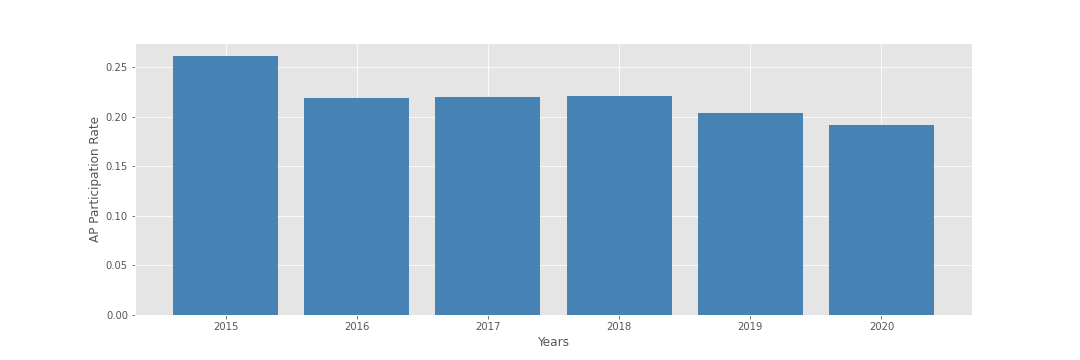
\includegraphics[width=10cm]{AP Participation Rate.png}
        \label{fig1}
    \end{figure}
\end{frame}

\begin{frame}{}
    \begin{figure}
        \caption{AP Pass Rate over Time}
        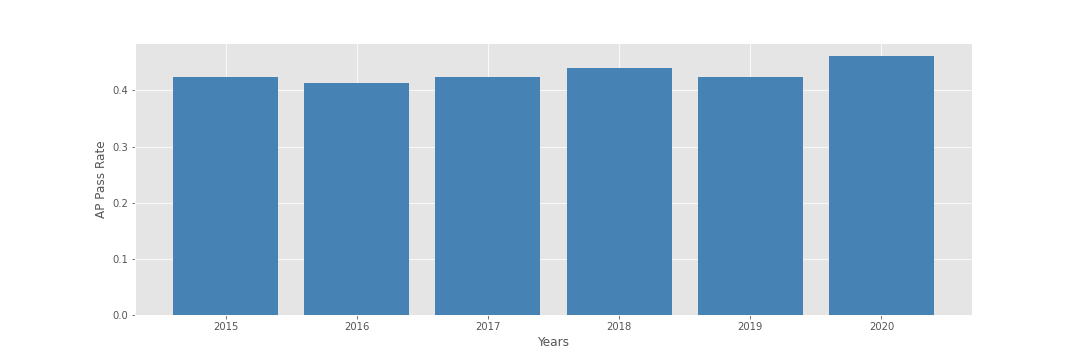
\includegraphics[width=11cm]{AP Pass Rate.png}
        \label{fig2}
    \end{figure}     
\end{frame}
    
\begin{frame}{}
    \begin{figure}
        \caption{Economically Disadvantaged Students College Enrollment over Time}
        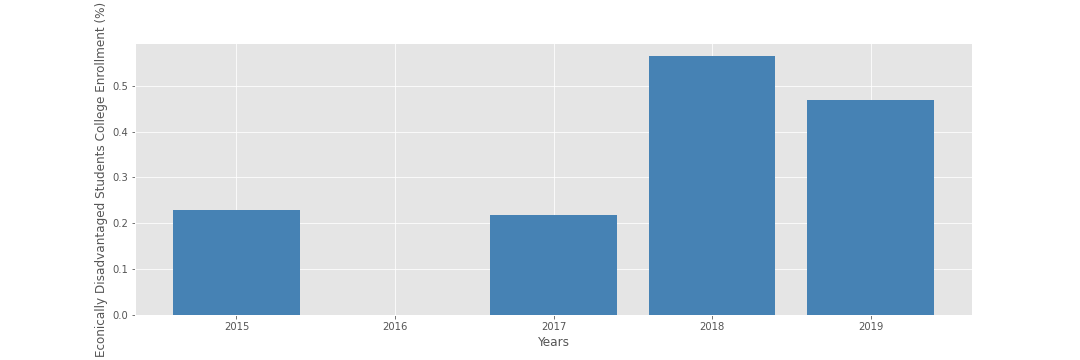
\includegraphics[width=11cm]{EDS Students College Enrollment.png}
        \label{fig4}
    \end{figure}
\end{frame}


\begin{frame}{}
    \begin{figure}
        \caption{CTE Student Enrollment over Time}
        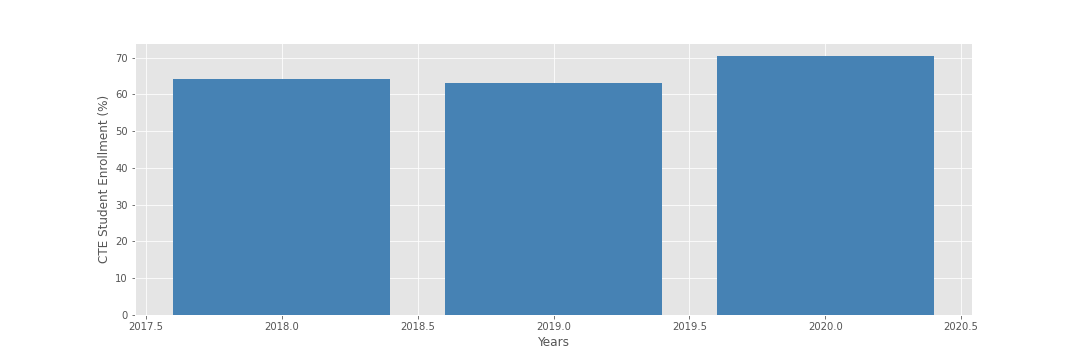
\includegraphics[width=11cm]{CTE Student Enrollment.png}
        \label{fig3}
    \end{figure}
\end{frame}

\begin{frame}{}
    \begin{figure}
        \caption{Number of Counselors at District Level}
        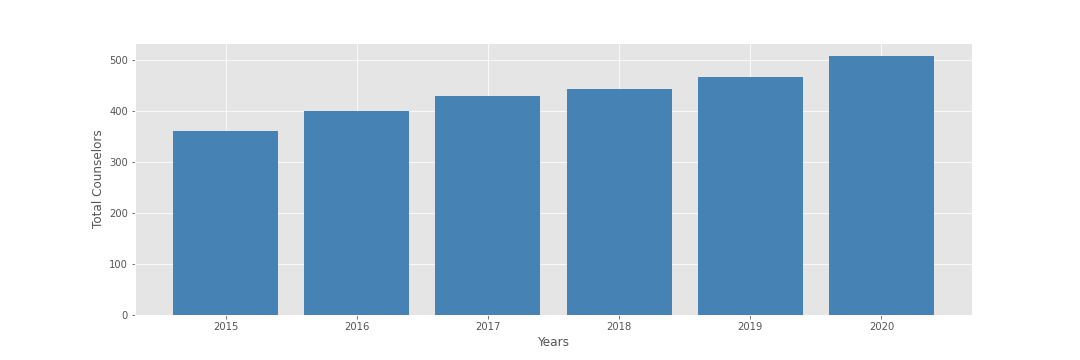
\includegraphics[width=11cm]{Total Counselors.png}
        \label{fig5}
    \end{figure}
\end{frame}



\end{document}
